% 2007 年湖北卷文科第 5 题：正方体 ABCD-A1B1C1D1，E、F 为 AA1、BB1 中点，
%   G 在 A1B1 上，平面 D1EF 与 G 的位置。
% 来源 PDF：gaokaomath-src/普通高考/2007/2007湖北文.pdf
% SHA-256：290a153da24ec0f3a3abb8bb916d9b7e06d203d3ef5bd7bb221c93f7f1b1cacb
% 原页：2007湖北文.pdf 第 1 页（A3 三栏）第 1 栏，书页码 377。
% 重绘依据：按原页正方体斜投影、E/F/G 与平面 D1EF 的虚实线重绘。
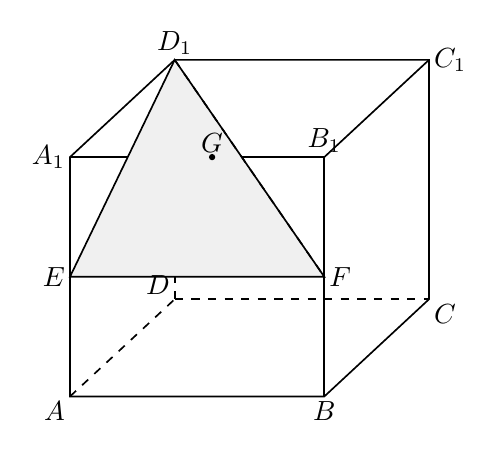
\begin{tikzpicture}[scale=0.95, semithick,
  every node/.style={inner sep=1.5pt}]
  \coordinate (A)  at (0,0);
  \coordinate (B)  at (3.4,0);
  \coordinate (C)  at (4.8,1.3);
  \coordinate (D)  at (1.4,1.3);
  \coordinate (A1) at (0,3.2);
  \coordinate (B1) at (3.4,3.2);
  \coordinate (C1) at (4.8,4.5);
  \coordinate (D1) at (1.4,4.5);
  \coordinate (E)  at (0,1.6);
  \coordinate (F)  at (3.4,1.6);
  \coordinate (G)  at (1.9,3.2);

  \draw[dashed] (A) -- (D);
  \draw[dashed] (D) -- (C);
  \draw[dashed] (D) -- (D1);
  \draw (A) -- (B) -- (C) -- (C1) -- (D1) -- (A1) -- cycle;
  \draw (A) -- (A1); \draw (B) -- (B1); \draw (C) -- (C1);
  \draw (A1) -- (B1); \draw (B1) -- (C1);
  % 平面 D1EF
  \fill[gray!12] (D1) -- (E) -- (F) -- cycle;
  \draw (D1) -- (E) -- (F) -- cycle;
  \draw[dashed] (D1) -- (F);
  \fill (G) circle (1.2pt);

  \node[below left] at (A) {$A$};
  \node[below] at (B) {$B$};
  \node[below right] at (C) {$C$};
  \node[above left] at (D) {$D$};
  \node[left] at (A1) {$A_1$};
  \node[above] at (B1) {$B_1$};
  \node[right] at (C1) {$C_1$};
  \node[above] at (D1) {$D_1$};
  \node[left] at (E) {$E$};
  \node[right] at (F) {$F$};
  \node[above] at (G) {$G$};
\end{tikzpicture}
